\documentclass[12pt,a4paper]{ufpr}

% \usepackage[portuges,brazil]{babel}
% \usepackage[portuguese,brazil]{babel}

\usepackage[brazilian]{babel}
\usepackage[latin1]{inputenc}
\usepackage[T1]{fontenc}
%\usepackage[brazil]{babel}
%\usepackage[latin1]{inputenc}
\usepackage{amssymb,amsmath}
\usepackage{epsfig}
\usepackage{multirow}

%\usepackage{isolatin1}
\usepackage{amssymb}
\usepackage{subfigure}
\usepackage{graphicx}
\usepackage{caption2}
\usepackage{setspace}
%\usepackage{ps-macros}
% \usepackage{psfig}

\setcounter{secnumdepth}{3}    % n - numero de niveis de subsubsection numeradas
\setcounter{tocdepth}{3}       % coloca ate o nivel n no sumario

\title{WiSync: Sincroniza��o de Diret�rios em LAN}
\author{Renan Domingos Merlin Greca}
\advisortitle{Orientador} % ou Orientador
\advisorname{Prof. Dr. Luiz Carlos P. Albini}
\advisorplace{Departamento de Inform�tica, UFPR}  % departamento, instituicao
\city{Curitiba}
\year{2015}

%\banca        % nao insira o nome do orientador, ja eh feito automaticamente
%{Prof. Dr. Luciano Fontoura}{Instituto de F�sica, USP}
%{Prof. Dr. H�lio Pedrini}{Departamento de Inform�tica, UFPR}
%{Prof. Dr. Alexandre I. Direne}{Departamento de Inform�tica, UFPR} % se nao houver deixe em branco {}{}
%{}{}    % se houver um quarto membro na banca, inserir nome e instituicao

%\defesa{04 de outubro de 2014} % dia em que foi realizada a defesa da dissertacao


\begin{document}

%\makecapaproposta             % cria capa para proposta%
\makecapadissertacao           % cria capa para dissertacao de mestrado %
\makerosto                     % cria folha de rosto para versao final da UFPR %
%\maketermo                     % cria folha com o termo de aprovacao da dissertacao%

%\singlespacing           % espacamento 1 - capa UFPR%
%\onehalfspacing          % espacamento 1/2 %
\doublespacing            % espacamento 2 - UFPR %

\pagestyle{headings}
\pagenumbering{roman}

\chapter*{Agradecimentos}
\input{agradecimentos.tex}          % possiu somente o texto

\tableofcontents

\listoffigures         % se houver mais do que 3 figuras
\addcontentsline{toc}{chapter}{\MakeUppercase{Lista de Figuras}}
\newpage

\listoftables        % se houver mais do que 3 tabelas
\addcontentsline{toc}{chapter}{\MakeUppercase{Lista de Tabelas}}
\newpage

\chapter*{Resumo}
\addcontentsline{toc}{chapter}{\MakeUppercase{Resumo}}
Texto do resumo....
           % somente o texto
\newpage

\chapter*{Abstract}
\addcontentsline{toc}{chapter}{\MakeUppercase{Abstract}}
Texto do abstract....
        % somente o texto
\newpage

\pagenumbering{arabic}

%\chapter*{Relat�rio de Final de Semestre}
%\begin{center}
%Renan Greca
%\end{center}

%\addcontentsline{toc}{chapter}{\MakeUppercase{Relat�rio de Final de Semestre}}
%O \textit{LAN para Sincroniza��o de Diret�rios} (daqui em diante abreviado como \textit{LSD}) ser� um programa multiplataforma para manter diret�rios sincronizados atrav�s de uma rede local (LAN - \textit{Local Area Network}).
Este relat�rio descreve o in�cio do projeto, desde a motiva��o da ideia at� os desenvolvimentos atuais.

A ideia do \textit{LSD} veio da necessidade de manter diret�rios em dois computadores pertencentes ao mesmo usu�rio sincronizados para oferecer conveni�ncia.
Por exemplo, ao chegar em casa com seu \textit{laptop}, os documentos novos neste seriam automaticamente copiados para o \textit{desktop} do usu�rio.
Portanto, essa ser� a funcionalidade principal do \textit{LSD}:
(1) Executa-se duas inst�ncias do programa em dois computadores em rede, cada uma recebendo um diret�rio como argumento;
(2) Os diret�rios s�o comparados e suas diferen�as s�o analisadas pelo programa;
(3) Arquivos s�o copiados de um diret�rio para outro at� que ambos sejam iguais.

O \textit{LSD} ser� desenvolvido na linguagem de programa��o Python, escolhida pelo seu desenvolvimento r�pido e facilidade de acesso a recursos de rede.
Com sockets TCP, � poss�vel efetuar comunica��o entre duas inst�ncias do programa atrav�s da rede local.
Por enquanto, dois prot�tipos est�o sendo desenvolvidos:
Um deles analisa um diret�rio e armazena a lista de arquivos (inclusive de sub-diret�rios) e as datas de cria��o e modifica��o desses;
outro envia arquivos espec�ficos de um computador a outro atrav�s da rede.
Quando ambos prot�tipos estiverem s�lidos, eles ser�o combinados para realizar a proposta do \textit{LSD}.

Abaixo est�o algumas poss�veis situa��es que podem ocorrer ao se comparar diret�rios (vamos cham�-los de A e B), e como pretende-se lidar com elas no \textit{LSD}:
\begin{enumerate}
	\item Um arquivo � encontrado no diret�rio A, mas n�o no diret�rio B. Neste caso, basta copiar esse arquivo de A para B. H� a possibilidade de que o arquivo j� existia e foi exclu�do de B. Portanto, � necess�rio comparar as informa��es de cada diret�rio com a de si mesmo durante a execu��o anterior do programa. 
	\item Um arquivo existe em ambos, mas n�o � igual. Deve-se comparar as datas de altera��o contidas nos metadados dos arquivos. H� a possibilidade de um ser apenas a atualiza��o do outro, mas pode ser que ambos sejam atualiza��es de uma vers�o comum anterior. Na eventualidade de um conflito, o programa dever� indagar o usu�rio sobre como prosseguir.
	\item Um arquivo foi renomeado em A mas n�o sofreu altera��es em B. Deve-se verificar qual foi era o nome original do arquivo renomeado e ent�o renome�-lo tamb�m em B.
\end{enumerate}
Durante o desenvolvimento do trabalho, outras situa��es podem ocorrer durante testes. Elas ser�o tratadas de forma adequada.

Nos pr�ximos meses, o foco do projeto ser� concluir e integrar os prot�tipos para poder efetuar a sincroniza��o.
Ap�s isso, num poss�vel passo adicional, ser� considerada a hip�tese de fazer com que o programa detecte automaticamente mudan�as no diret�rio para fazer a sincroniza��o em tempo real.
\newpage

\chapter{Introdu��o}
\label{Introducao}
Com o barateamento e a populariza��o de microcomputadores, � comum hoje um escrit�rio, uma fam�lia ou at� mesmo um indiv�duo ter diversos computadores pessoais � sua disposi��o.
Portanto, torna-se �til e �s vezes necess�rio existir uma maneira de manter esses computadores ``conversando'' entre si, trocando informa��es e arquivos para que o usu�rio possa mudar de um para outro de forma coesa.
Al�m disso, computadores port�teis (i.e., \textit{laptops}) s�o mais vulner�veis do que computadores dom�sticos a roubos ou danos f�sicos, al�m de outros fatores que podem comprometer a integridade das informa��es neles contidas, o que torna necess�ria a realiza��o de \textit{backups} frequentes.

\section{Proposta}
Para trabalhar em diversos computadores ou manter c�pias seguras de arquivos de forma conveniente, o presente projeto prop�e um programa que, atrav�s de uma rede local (daqui em diante referida como LAN, de \textit{Local Area Network}), compare diret�rios em dois ou mais computadores distintos e realize a sincroniza��o dos mesmos.
Com sincroniza��o, queremos dizer que o programa ir�, para cada inst�ncia rodando:
\begin{itemize}
    \item Copiar arquivos novos (adicionados desde a �ltima execu��o) �s outras inst�ncias;
    \item Apagar arquivos removidos nas outras inst�ncias; e
    \item Copiar altera��es aos arquivos �s outras inst�ncias, incluindo arquivos renomeados.
\end{itemize}

\section{Trabalhos Similares}
Atualmente existem alguns programas dispon�veis na Internet que fazem opera��es desse tipo, apesar de que em contextos um pouco diferentes.

Entre produtos comerciais, h� diversos servi�os de armazenamento em nuvem que suportam a sincroniza��o de diret�rios caso o usu�rio instale um aplicativo em cada computador.
Exemplos desses produtos incluem Dropbox \cite{dropbox}, Box \cite{box}, Google Drive \cite{googledrive}, Apple iCloud Drive \cite{icloud} e Microsoft OneDrive \cite{onedrive}.
A principal diferen�a desses produtos ao atual projeto � a exist�ncia de um servidor mantendo os arquivos na ``nuvem''.
A vantagem dessa decis�o � que o usu�rio pode acessar seus arquivos facilmente de outros dispositivos como celulares e tablets \-- contudo, para a sincroniza��o ocorrer � necess�rio que os computadores clientes estejam conectados � Internet e todos esses servi�os imp�em limites em bytes na quantidade de arquivos que podem ser sincronizados.

Outra categoria de programas que realizam opera��es semelhantes s�o os programas de \textit{backup}.
Um exemplo desses programas � o FreeFileSync \cite{freefilesync}, solu��o \textit{open-source} dispon�vel na web.
Dados um par de diret�rios A e B, programas de \textit{backup} normalmente possuem tr�s funcionalidades:
\begin{itemize}
    \item Sincroniza��o de dois sentidos, que torna A e B id�nticos copiando as modifica��es de um para o outro e vice-versa;
    \item Sincroniza��o de espelho, que faz o diret�rio B ser um clone do diret�rio A, incluindo arquivos removidos; e
    \item Sincroniza��o de atualiza��o, que atualiza B com os arquivos novos ou modificados de A, mas n�o remove arquivos exclu�dos em A.

Para o prop�sito desta monografia, o projeto ir� focar no primeiro tipo de sincroniza��o, a de dois sentidos.
Os outros dois tipos s�o interessantes e possivelmente ser�o adicionados ao escopo futuramente.
\end{itemize}


% *****************
% O [41] determina o percentual de reducao em relacao ao tamanho original.
% *****************
%\begin{figure}
%\centerfig{feature_space_2D.ps}[41]
%\caption{Legenda geral da figura.}
%\label{figura_xpto}
%\end{figure}
% *****************

% *****************
% O .50 da minipage e' para dividir a largura da pagina em 2 figuras por
% linhas, se for colocar 3 subfiguras por linha .33 e assi vai...
% a largura da imagem e' 3cm.(width=3cm).
%
% O (!ht) e' para forcar o latex a colocar a figura na posicao, ou
% paragrafo onde foi inserido no texto o \begin{figure}, "se possivel"
% e' claro...
% *****************
%\begin{figure}[!ht]
%\renewcommand{\captionfont}{\it}
%\renewcommand{\captionlabelfont}{\bf}
%\begin{minipage}[b]{.50\textwidth}
%\centering
%  \subfigure[Imagem 1]{
%    \label{fig:teste:a}
%    \includegraphics[width=3cm]{feature_space_2D.ps}}
%\end{minipage}%
%\begin{minipage}[b]{.50\textwidth}
%\centering
%  \subfigure[Imagem 2]{
%    \label{fig:teste:b}
%    \includegraphics[width=3cm]{feature_space_2D.ps}}
%\end{minipage}
%\caption{
%  Legenda geral da figura contendo 2 sub-figuras colocadas lado a lado.}
%\label{fig:teste}
%\end{figure}
% *****************

% *****************
%\begin{figure}
%\psfig{file=feature_space_2D.ps,height=2in,width=3.5in}
%\caption{Legenda geral da figura usando psfig COM reducao.}
%\end{figure}
% *****************

% *****************
%\begin{figure}
%\psfig{file=feature_space_2D.ps}
%\caption{Legenda geral da figura usando psfig SEM reducao.}
%\end{figure}
% *****************

\chapter{Implementa��o}
\label{Implementacao}
Neste cap�tulo, ser� descrita a implementa��o do \textbf{WiSync} para este trabalho.

A vers�o do \textbf{WiSync} entregue com este texto foi escrita em Python \cite{python}, vers�o 2.7, linguagem de programa��o interpretada originalmente lan�ada em 1991. Python foi escolhida por sua facilidade na implementa��o e extensa disponibilidade de bibliotecas de c�digo aberto.

Originalmente, havia como objetivo tornar o programa compat�vel com os tr�s sistemas operacionais mais comuns do mundo: Microsoft Windows, Apple OS X e Linux. Contudo, devido a diferen�as inerentes na forma como o Windows funciona, optou-se por manter apenas compatibilidade com OS X e Linux. Para tal, foram usados os seguintes computadores de teste:

\begin{center}
  \begin{tabular}{ l | l | l }
    \hline
    \textbf{Nome} & ``SgtPepper'' & ``Packard'' \\ \hline \hline
    Sistema Operacional & OS X 10.10 & Linux Mint 17 \\ \hline
    Processador & Intel Core i5-4308U & Intel Core i7-2600 \\ \hline
    RAM & 8GB DDR3L & 8GB DDR3 \\ \hline
    Conectividade & Wi-fi 802.11n 5GHz & Cabo Ethernet \\ \hline
    IP local & 192.168.1.110 & 192.168.1.132 \\
    \hline
  \end{tabular}
\end{center}

\section{Organiza��o do Programa}
Na vers�o atual, o WiSync � composto por tr�s arquivos: \texttt{wisync.py}, \texttt{winet.py} e \texttt{wifiles.py}. Abaixo est�o as funcionalidades de cada um:
\begin{itemize}
	\item \texttt{wisync.py}: Arquivo principal do projeto, respons�vel por ler os par�metros da linha de comando e controlar a execu��o do processo.
	\item \texttt{winet.py}: Cont�m a classe WiNet, que inclui os m�todos e atributos necess�rios para fazer as partes em rede do programa, como hospedar e receber arquivos.
	\item \texttt{wifiles.py}: Cont�m a classe WiFiles, que inclui os m�todos e atributos necess�rios fazer as partes que lidam com o sistema de arquivos do programa, como ler e comparar diret�rios.
\end{itemize}

Para executar o \textbf{WiSync}, s�o necess�rias algumas bibliotecas padr�o do Python: \texttt{os}, \texttt{sys}, \texttt{argparse}, \texttt{time}, \texttt{json}, \texttt{datetime}. Tamb�m � usada uma vers�o modificada do programa \texttt{woof.py} \cite{woof} (distribu�da sob a licen�a GNU General Public License), que � usada na hora de transmitir os arquivos entre os computadores.

\section{Sobre a Transmiss�o dos Arquivos}
A primeira etapa do desenvolvimento do programa foi definir o m�todo e protocolo que seriam usados na hora de transmitir arquivos entre os computadores. Ap�s alguma pesquisa, quatro alternativas foram consideradas: sockets via TCP, FTP, SCP e HTTP.
\input{capitulo3.tex}
%\input{capitulo4.tex}
%\input{capitulo5.tex}
%\input{capitulo6.tex}
%\input{anexo1.tex}     % se houver anexo



\bibliographystyle{brazil}
\bibliography{dissertacao}
% utilize macros (3 primeiras letras do mes em ingles, minusculas) no seu
% .bib para atribuir o nome do mes em portugues nas referencia,
% se o style for brazil, outros estilos tambem aceitam estas macros
% Ex:
%
% @InProceedings{teste,
%   author =       {Luciano}
%   year =         {2000}
%   month =        {}#sep;
% }
%
\addcontentsline{toc}{chapter}{\MakeUppercase{Bibliografia}}

\singlespacing
\makecapadissertacao

\end{document}
